\documentclass[12pt,a4paper]{article}

% --- PAKIETY JĘZYKOWE I KODOWANIE ---
\usepackage[T1]{fontenc}
\usepackage[utf8]{inputenc}
\usepackage[polish]{babel} % Dodaj to, jeśli piszesz po polsku (ładne przenoszenie wyrazów)

% --- GEOMETRIA STRONY ---
\usepackage[a4paper, total={7.5in, 9in}]{geometry}

% --- MATEMATYKA I SYMBOLE ---
\usepackage{amsmath}
\usepackage{amssymb}
\usepackage{gensymb} % Symbole typu stopnie itp.

% --- GRAFIKA I POZYCJONOWANIE ---
\usepackage{graphicx} 
\usepackage{float} % Pozwala użyć [H] przy obrazkach
\usepackage{caption}
\usepackage{subcaption}
% Uwaga: subfig i subcaption czasem się gryzą. Lepiej trzymać się subcaption.

% --- TABELE ---
\usepackage{multirow}
\usepackage{array}
\usepackage[table, dvipsnames]{xcolor} % Poprawione dvipsnames

% --- TYPOGRAFIA I WYGLĄD ---
\usepackage{microtype}
\usepackage{titlesec}
\title{Wprowadzenie do napędu BLDC}
\author{Zuzanna Andrzejak, Jan Andrzejewski, Mateusz Banaszak}
\date{}


\begin{document}
\maketitle

\section{Omówienie modelu silnika BLDC}
W środowisku LTSpice część mechaniczna została podzielona na dwa powiązane ze sobą bloki obwodowe, 
realizujące odpowiednio równanie dynamiki ruchu obrotowego oraz równanie kinematyczne. 
Wykorzystano tu bezpośrednią analogię elektromechaniczną, w której momenty obrotowe 
reprezentowane są przez źródła prądowe, prędkość i położenie przez napięcia w danych miejscach obwodu, 
moment bezwładności przez kondensator, a współczynnik tarcia przez rezystancję.

\subsection{Obwód dynamiki wirnika}

\begin{figure}[H]
    \centering
    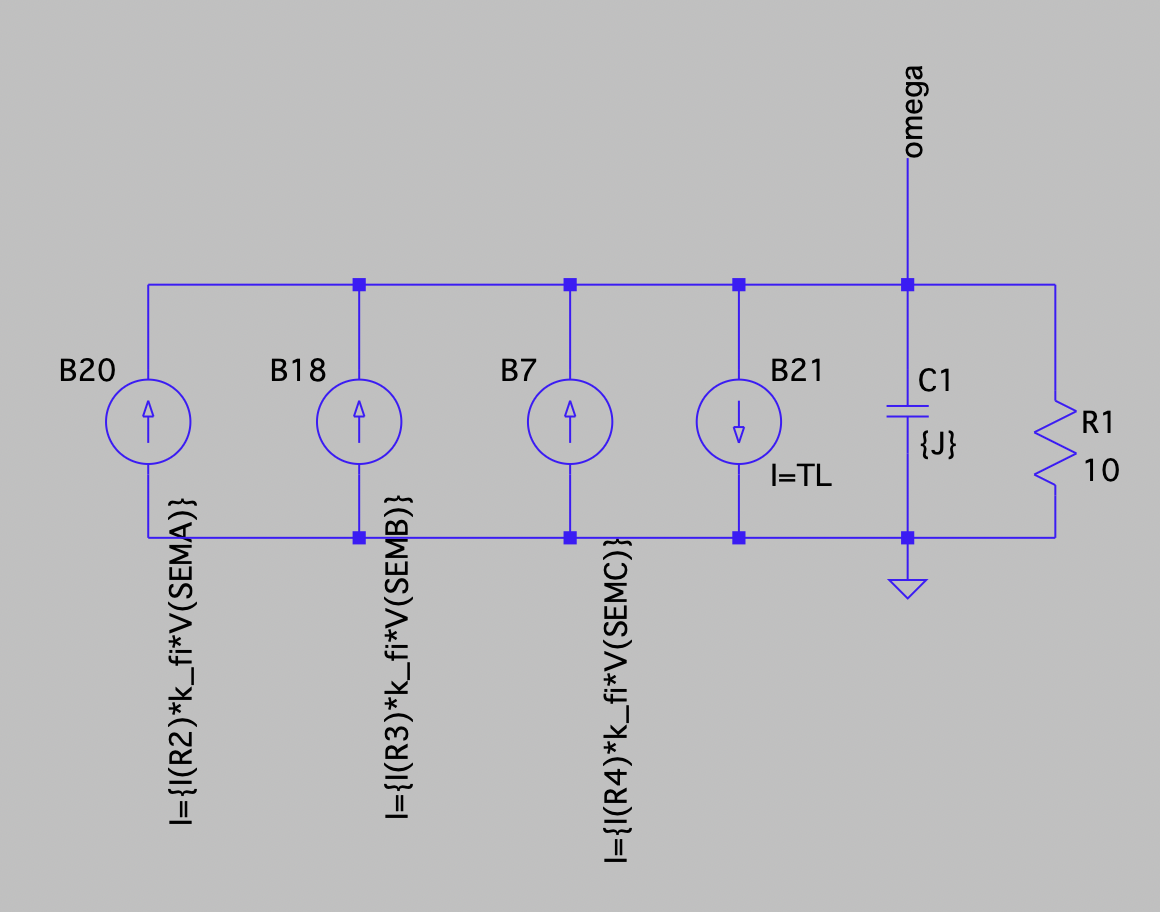
\includegraphics[width=0.8\textwidth]{images/dynamika_wirnika.png}
    \caption{Obwód przedstawiający dynamikę ruchu obrotowego.}
    \label{fig:unikalna_nazwa}
\end{figure}

Ten fragment układu rozwiązuje równanie dynamiki Newtona dla ruchu obrotowego:

\[
T_{em}- T_{L}= J \cdot \frac{d\omega_{m}}{dt} + B \omega_{m}
\]
Układ opiera się na sumowaniu prądów w głównym węźle omega, którego potencjał (napięcie) jest analogiem prędkości kątowej maszyny $\omega_m$. 
Poszczególne elementy obwodu pełnią następujące funkcje:

\begin{itemize}
    \item \textbf{Źródła sterowane (B20, B18, B7):} Dają prądy, które są wprost proporcjonalne do momentów elektromagnetycznych generowanych przez poszczególne fazy silnika (obliczanych na podstawie siły elektromotorycznej i prądu fazowego).

    \item \textbf{Źródło prądowe B21 ($I = T_L$):} Symuluje moment obciążenia na wale silnika. Zabiera prąd z węzła \texttt{omega}, co prowadzi do spadku wyliczanego napięcia, które symbolizuje spadek prędkości.

    \item \textbf{Kondensator C1 ($\{J\}$):} Pełni rolę mechanicznego momentu bezwładności wirnika~($J$). Czas jego ładowania odzwierciedla bezwładność maszyny podczas rozruchu i zmian obciążenia.

    \item \textbf{Rezystor R1:} Reprezentuje straty mechaniczne, takie jak tarcie ($B$). Odprowadza część prądu do masy, symbolizując rozproszenie energii i ograniczając maksymalną prędkość silnika w stanie ustalonym.
\end{itemize}



\subsection{Układ całkujący (wyznaczanie położenia kątowego)}

\begin{figure}[H]
    \centering
    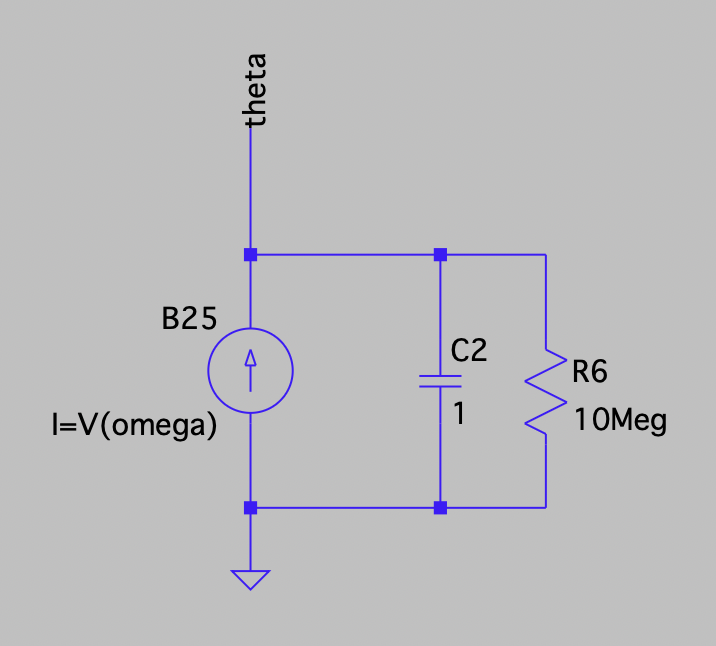
\includegraphics[width=0.5\textwidth]{images/polozenie_katowe.png}
    \caption{Obwód całkujący wyznaczania położenia kątowego wirnika}
    \label{fig:obwod_caltkujacy}
\end{figure}

Drugi obwód realizuje równanie kinematyczne. Jego zadaniem jest całkowanie w czasie wyliczonej wcześniej prędkości kątowej, co pozwala na bieżąco określać elektryczne położenie kątowe wirnika~$\theta_e$.

\begin{itemize}
    \item \textbf{Źródło B25 ($I = V(\texttt{omega})$):} Jest to źródło prądowe sterowane napięciem. Jest źródłem prądu o wartości liczbowo równej wyliczonej prędkości obrotowej z węzła~\texttt{omega} wylicoznej z poprzedniego obwodu.

    \item \textbf{Kondensator C2:} Element pełniący funkcję całkującą  prąd ze źródła B25. Odkładające się na nim napięcie w węźle \texttt{theta} jest wprost proporcjonalne do pokonanego przez wirnik kąta.

    \item \textbf{Rezystor R6 (10\,M$\Omega$):} Ma bardzo dużą rezystancję i z punktu widzenia fizyki modelowanej maszyny jest całkowicie pomijalny. Został dodany wyłącznie w celu stabilizacji obliczeniowej symulatora LTSpice.
\end{itemize}

\section{Praca "prądnicowa" silnika}
\subsection{napięcie fazowe i miedzyfazowe}


\subsection{Sygnały czujników Halla}

\subsection{Prędkość i położenie}

\end{document}